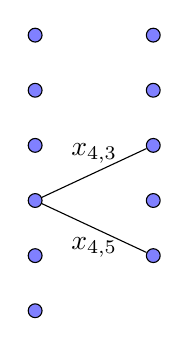
\begin{tikzpicture}[>=latex]

    \foreach \i in {1, 2, ..., 6}{
        \node[draw, circle, fill = blue!50, inner sep = 0pt, minimum size = 5pt]
            (a\i) at (0, -0.7 * \i) {};
    }

    \foreach \i in {1, 2, ..., 5}{
        \node[draw, circle, fill = blue!50, inner sep = 0pt, minimum size = 5pt]
            (b\i) at (1.5, -0.7 * \i) {};
    }
    
    \draw (a4) -- (b3) node[midway, above] {$x_{4, 3}$};
    \draw (a4) -- (b5) node[midway, below] {$x_{4, 5}$};
\end{tikzpicture}